\documentclass[tikz,border=12pt]{standalone}
\usepackage[utf8]{inputenc}
\usepackage[T1]{fontenc}
\usepackage{lmodern}
\usepackage{array}
\usepackage{tikz}
\usetikzlibrary{arrows.meta,calc}
\definecolor{greenFill}{HTML}{E8F5E9}
\definecolor{greenStroke}{HTML}{43A047}
\definecolor{coreFill}{HTML}{E1F5FE}
\definecolor{coreStroke}{HTML}{0277BD}
\newcommand{\classcontent}[2]{\begin{tabular}{p{5.8cm}}\centering\bfseries #1\tabularnewline\hline\raggedright\arraybackslash #2\end{tabular}}
\begin{document}
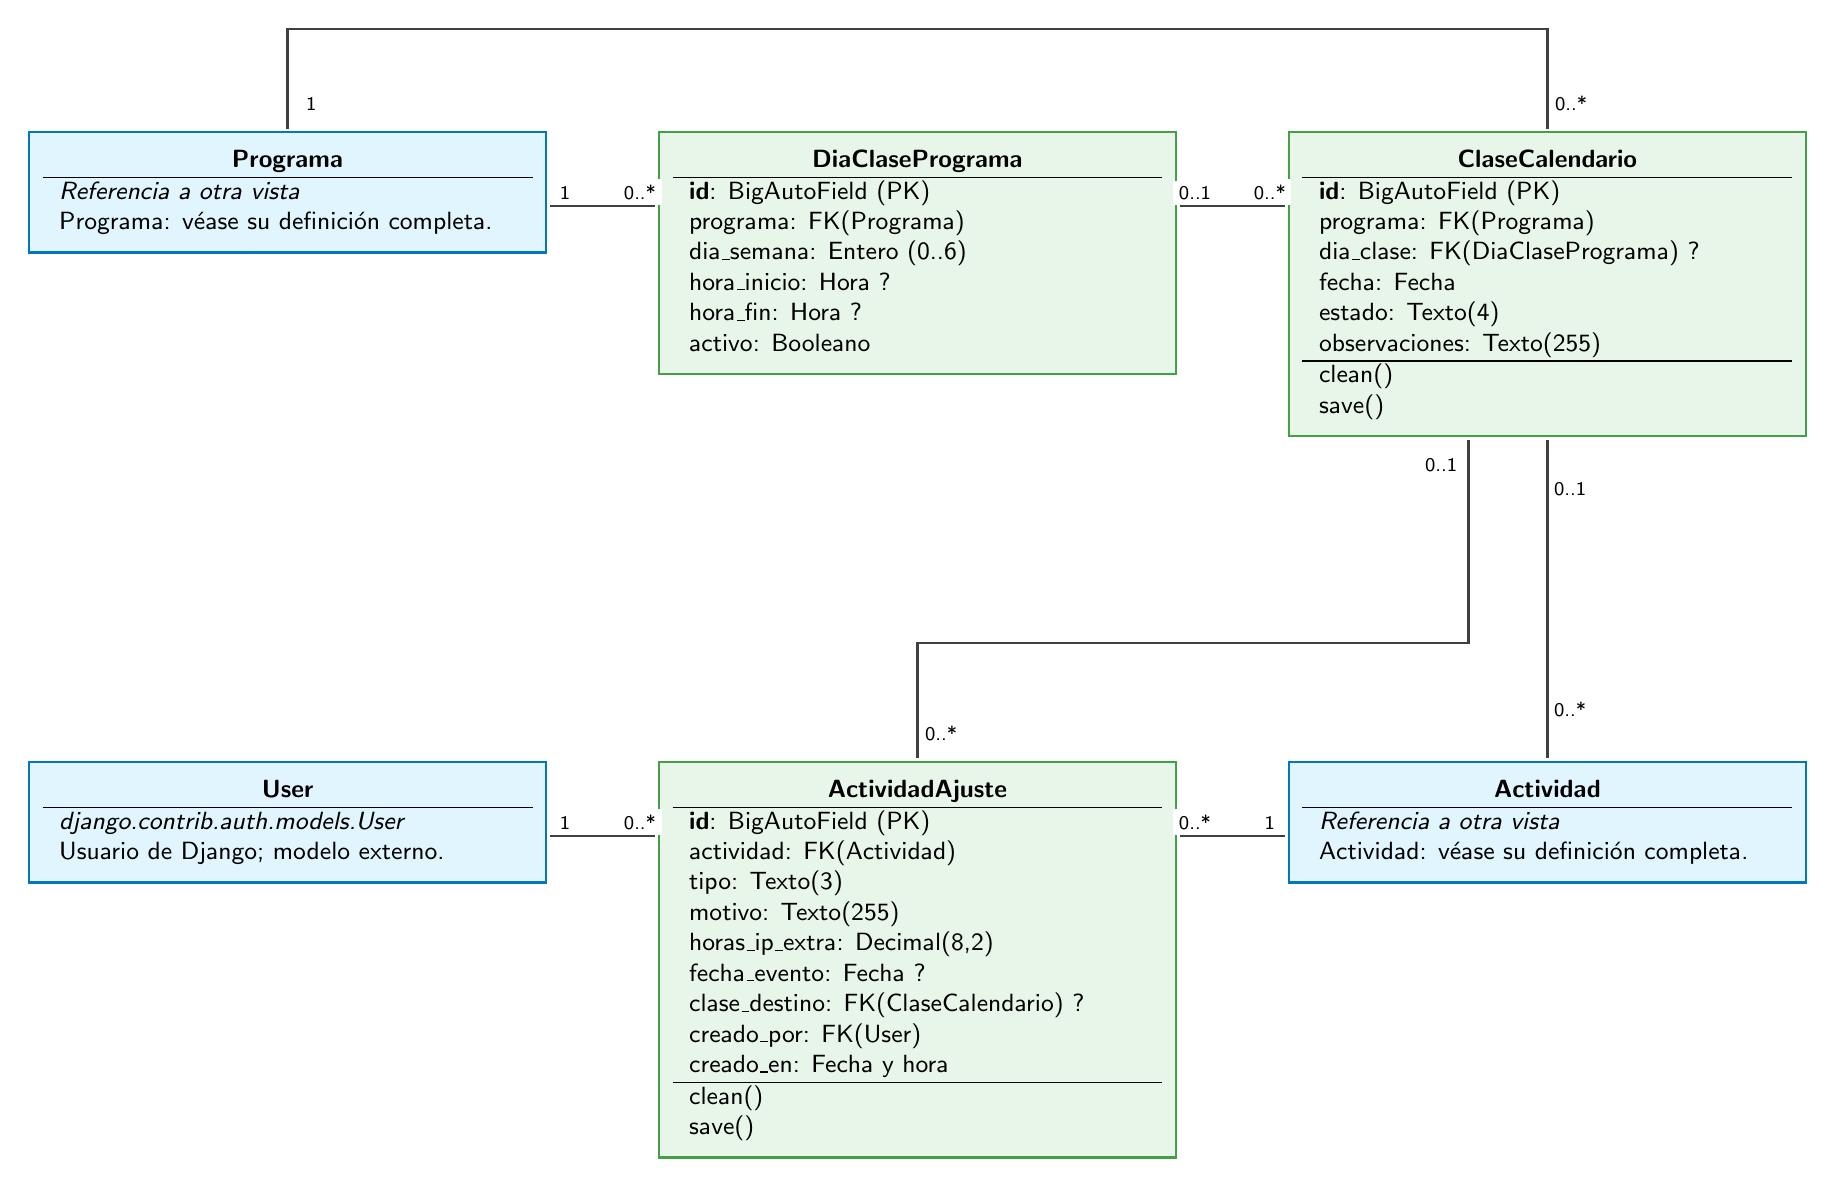
\begin{tikzpicture}[
 font=\sffamily\small,
 cls/.style={rectangle,draw=greenStroke,fill=greenFill,line width=.8pt,inner sep=5pt,anchor=north},
 ref/.style={cls,draw=coreStroke,fill=coreFill},
 association/.style={line width=.9pt,draw=black!75,shorten >=1pt,shorten <=1pt},
 dependency/.style={association,dashed,-{Stealth[length=3mm,width=2.2mm]}},
 mult/.style={font=\sffamily\scriptsize,fill=white,inner sep=2pt,text=black}
]
\node[ref] (Programa) at (0,0) {\classcontent{Programa}{\textit{Referencia a otra vista}\\Programa: véase su definición completa.}};
\node[cls] (DiaClasePrograma) at (8,0) {\classcontent{DiaClasePrograma}{\textbf{id}: BigAutoField (PK)\\programa: FK(Programa)\\dia\_semana: Entero (0..6)\\hora\_inicio: Hora ?\\hora\_fin: Hora ?\\activo: Booleano}};
\node[cls] (ClaseCalendario) at (16,0) {\classcontent{ClaseCalendario}{\textbf{id}: BigAutoField (PK)\\programa: FK(Programa)\\dia\_clase: FK(DiaClasePrograma) ?\\fecha: Fecha\\estado: Texto(4)\\observaciones: Texto(255)\\\hline clean()\\save()}};
\node[ref] (User) at (0,-8) {\classcontent{User}{\textit{django.contrib.auth.models.User}\\Usuario de Django; modelo externo.}};
\node[cls] (ActividadAjuste) at (8,-8) {\classcontent{ActividadAjuste}{\textbf{id}: BigAutoField (PK)\\actividad: FK(Actividad)\\tipo: Texto(3)\\motivo: Texto(255)\\horas\_ip\_extra: Decimal(8,2)\\fecha\_evento: Fecha ?\\clase\_destino: FK(ClaseCalendario) ?\\creado\_por: FK(User)\\creado\_en: Fecha y hora\\\hline clean()\\save()}};
\node[ref] (Actividad) at (16,-8) {\classcontent{Actividad}{\textit{Referencia a otra vista}\\Actividad: véase su definición completa.}};
\draw[association] ($(Programa.north east)+(0,-.95)$) -- ($(DiaClasePrograma.north west)+(0,-.95)$) node[pos=.16,above,mult]{1} node[pos=.84,above,mult]{0..*};
\draw[association] ($(DiaClasePrograma.north east)+(0,-.95)$) -- ($(ClaseCalendario.north west)+(0,-.95)$) node[pos=.16,above,mult]{0..1} node[pos=.84,above,mult]{0..*};
\draw[association] (Programa.north) -- (0,1.3) -- (16,1.3) -- (ClaseCalendario.north);
\node[mult] at ($(Programa.north)+(.3,.35)$) {1};
\node[mult] at ($(ClaseCalendario.north)+(.3,.35)$) {0..*};
\draw[association] (ClaseCalendario.south) -- (Actividad.north) node[pos=.16,right,mult]{0..1} node[pos=.84,right,mult]{0..*};
\draw[association] ($(Actividad.north west)+(0,-.95)$) -- ($(ActividadAjuste.north east)+(0,-.95)$) node[pos=.16,above,mult]{1} node[pos=.84,above,mult]{0..*};
\draw[association] ($(User.north east)+(0,-.95)$) -- ($(ActividadAjuste.north west)+(0,-.95)$) node[pos=.16,above,mult]{1} node[pos=.84,above,mult]{0..*};
\draw[association] ($(ClaseCalendario.south)+(-1,0)$) -- (15,-6.5) -- (8,-6.5) -- (ActividadAjuste.north);
\node[mult] at ($(ClaseCalendario.south)+(-1.35,-.35)$) {0..1};
\node[mult] at ($(ActividadAjuste.north)+(.3,.35)$) {0..*};
\end{tikzpicture}
\end{document}
